% Created by tikzDevice version 0.12.3.1 on 2022-05-04 13:36:34
% !TEX encoding = UTF-8 Unicode
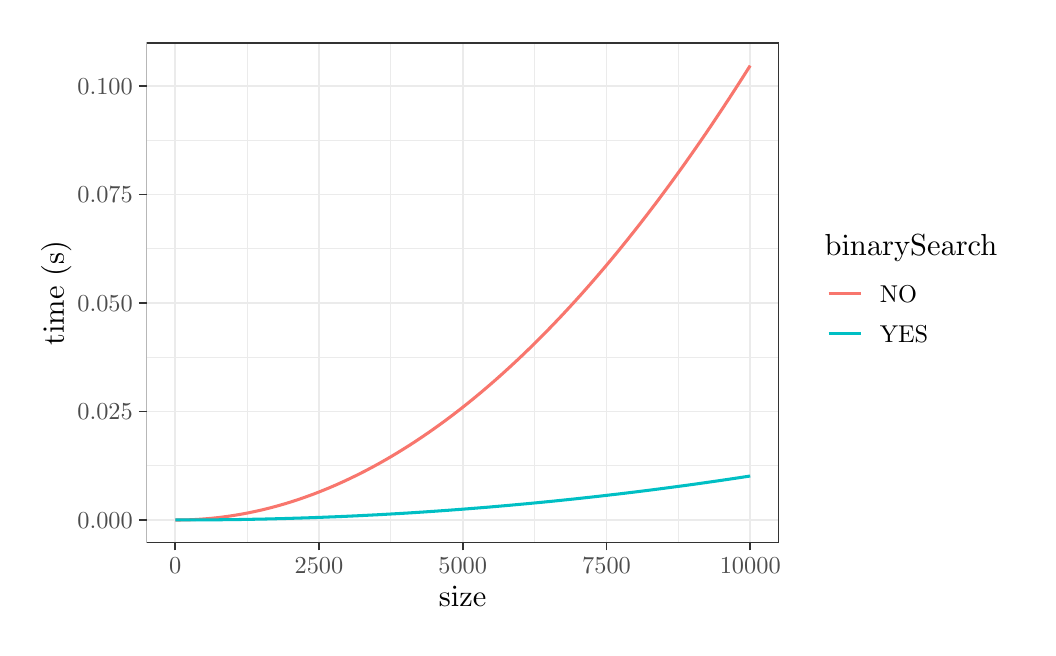
\begin{tikzpicture}[x=1pt,y=1pt]
\definecolor{fillColor}{RGB}{255,255,255}
\path[use as bounding box,fill=fillColor,fill opacity=0.00] (0,0) rectangle (361.35,216.81);
\begin{scope}
\path[clip] (  0.00,  0.00) rectangle (361.35,216.81);
\definecolor{drawColor}{RGB}{255,255,255}
\definecolor{fillColor}{RGB}{255,255,255}

\path[draw=drawColor,line width= 0.6pt,line join=round,line cap=round,fill=fillColor] (  0.00,  0.00) rectangle (361.35,216.81);
\end{scope}
\begin{scope}
\path[clip] ( 42.95, 30.69) rectangle (271.47,211.31);
\definecolor{fillColor}{RGB}{255,255,255}

\path[fill=fillColor] ( 42.95, 30.69) rectangle (271.47,211.31);
\definecolor{drawColor}{gray}{0.92}

\path[draw=drawColor,line width= 0.3pt,line join=round] ( 42.95, 58.47) --
	(271.47, 58.47);

\path[draw=drawColor,line width= 0.3pt,line join=round] ( 42.95, 97.68) --
	(271.47, 97.68);

\path[draw=drawColor,line width= 0.3pt,line join=round] ( 42.95,136.90) --
	(271.47,136.90);

\path[draw=drawColor,line width= 0.3pt,line join=round] ( 42.95,176.11) --
	(271.47,176.11);

\path[draw=drawColor,line width= 0.3pt,line join=round] ( 79.29, 30.69) --
	( 79.29,211.31);

\path[draw=drawColor,line width= 0.3pt,line join=round] (131.24, 30.69) --
	(131.24,211.31);

\path[draw=drawColor,line width= 0.3pt,line join=round] (183.19, 30.69) --
	(183.19,211.31);

\path[draw=drawColor,line width= 0.3pt,line join=round] (235.13, 30.69) --
	(235.13,211.31);

\path[draw=drawColor,line width= 0.6pt,line join=round] ( 42.95, 38.86) --
	(271.47, 38.86);

\path[draw=drawColor,line width= 0.6pt,line join=round] ( 42.95, 78.08) --
	(271.47, 78.08);

\path[draw=drawColor,line width= 0.6pt,line join=round] ( 42.95,117.29) --
	(271.47,117.29);

\path[draw=drawColor,line width= 0.6pt,line join=round] ( 42.95,156.51) --
	(271.47,156.51);

\path[draw=drawColor,line width= 0.6pt,line join=round] ( 42.95,195.72) --
	(271.47,195.72);

\path[draw=drawColor,line width= 0.6pt,line join=round] ( 53.32, 30.69) --
	( 53.32,211.31);

\path[draw=drawColor,line width= 0.6pt,line join=round] (105.27, 30.69) --
	(105.27,211.31);

\path[draw=drawColor,line width= 0.6pt,line join=round] (157.21, 30.69) --
	(157.21,211.31);

\path[draw=drawColor,line width= 0.6pt,line join=round] (209.16, 30.69) --
	(209.16,211.31);

\path[draw=drawColor,line width= 0.6pt,line join=round] (261.10, 30.69) --
	(261.10,211.31);
\definecolor{drawColor}{RGB}{248,118,109}

\path[draw=drawColor,line width= 1.1pt,line join=round] ( 53.34, 38.90) --
	( 55.97, 38.92) --
	( 58.60, 38.99) --
	( 61.23, 39.12) --
	( 63.86, 39.30) --
	( 66.49, 39.53) --
	( 69.12, 39.81) --
	( 71.75, 40.15) --
	( 74.38, 40.54) --
	( 77.01, 40.98) --
	( 79.64, 41.47) --
	( 82.27, 42.02) --
	( 84.90, 42.61) --
	( 87.53, 43.26) --
	( 90.16, 43.97) --
	( 92.79, 44.72) --
	( 95.42, 45.53) --
	( 98.05, 46.39) --
	(100.67, 47.31) --
	(103.30, 48.27) --
	(105.93, 49.29) --
	(108.56, 50.36) --
	(111.19, 51.48) --
	(113.82, 52.66) --
	(116.45, 53.89) --
	(119.08, 55.17) --
	(121.71, 56.50) --
	(124.34, 57.89) --
	(126.97, 59.32) --
	(129.60, 60.81) --
	(132.23, 62.36) --
	(134.86, 63.96) --
	(137.49, 65.60) --
	(140.12, 67.30) --
	(142.75, 69.06) --
	(145.38, 70.86) --
	(148.01, 72.72) --
	(150.64, 74.63) --
	(153.27, 76.60) --
	(155.90, 78.62) --
	(158.53, 80.69) --
	(161.16, 82.82) --
	(163.79, 85.00) --
	(166.42, 87.23) --
	(169.05, 89.52) --
	(171.68, 91.86) --
	(174.30, 94.25) --
	(176.93, 96.69) --
	(179.56, 99.19) --
	(182.19,101.74) --
	(184.82,104.35) --
	(187.45,107.00) --
	(190.08,109.72) --
	(192.71,112.48) --
	(195.34,115.30) --
	(197.97,118.17) --
	(200.60,121.09) --
	(203.23,124.07) --
	(205.86,127.10) --
	(208.49,130.18) --
	(211.12,133.32) --
	(213.75,136.51) --
	(216.38,139.76) --
	(219.01,143.06) --
	(221.64,146.41) --
	(224.27,149.82) --
	(226.90,153.27) --
	(229.53,156.79) --
	(232.16,160.35) --
	(234.79,163.97) --
	(237.42,167.64) --
	(240.05,171.37) --
	(242.68,175.15) --
	(245.31,178.98) --
	(247.94,182.87) --
	(250.56,186.81) --
	(253.19,190.80) --
	(255.82,194.85) --
	(258.45,198.95) --
	(261.08,203.10);
\definecolor{drawColor}{RGB}{0,191,196}

\path[draw=drawColor,line width= 1.1pt,line join=round] ( 53.34, 38.92) --
	( 55.97, 38.92) --
	( 58.60, 38.92) --
	( 61.23, 38.93) --
	( 63.86, 38.94) --
	( 66.49, 38.96) --
	( 69.12, 38.99) --
	( 71.75, 39.02) --
	( 74.38, 39.05) --
	( 77.01, 39.09) --
	( 79.64, 39.14) --
	( 82.27, 39.19) --
	( 84.90, 39.24) --
	( 87.53, 39.30) --
	( 90.16, 39.37) --
	( 92.79, 39.44) --
	( 95.42, 39.52) --
	( 98.05, 39.60) --
	(100.67, 39.68) --
	(103.30, 39.78) --
	(105.93, 39.87) --
	(108.56, 39.98) --
	(111.19, 40.08) --
	(113.82, 40.19) --
	(116.45, 40.31) --
	(119.08, 40.43) --
	(121.71, 40.56) --
	(124.34, 40.70) --
	(126.97, 40.83) --
	(129.60, 40.98) --
	(132.23, 41.13) --
	(134.86, 41.28) --
	(137.49, 41.44) --
	(140.12, 41.61) --
	(142.75, 41.78) --
	(145.38, 41.96) --
	(148.01, 42.14) --
	(150.64, 42.33) --
	(153.27, 42.52) --
	(155.90, 42.72) --
	(158.53, 42.92) --
	(161.16, 43.13) --
	(163.79, 43.34) --
	(166.42, 43.55) --
	(169.05, 43.78) --
	(171.68, 44.01) --
	(174.30, 44.24) --
	(176.93, 44.48) --
	(179.56, 44.72) --
	(182.19, 44.97) --
	(184.82, 45.22) --
	(187.45, 45.48) --
	(190.08, 45.74) --
	(192.71, 46.01) --
	(195.34, 46.29) --
	(197.97, 46.56) --
	(200.60, 46.85) --
	(203.23, 47.14) --
	(205.86, 47.43) --
	(208.49, 47.73) --
	(211.12, 48.04) --
	(213.75, 48.34) --
	(216.38, 48.66) --
	(219.01, 48.98) --
	(221.64, 49.30) --
	(224.27, 49.63) --
	(226.90, 49.97) --
	(229.53, 50.31) --
	(232.16, 50.66) --
	(234.79, 51.01) --
	(237.42, 51.36) --
	(240.05, 51.72) --
	(242.68, 52.09) --
	(245.31, 52.46) --
	(247.94, 52.84) --
	(250.56, 53.22) --
	(253.19, 53.61) --
	(255.82, 54.00) --
	(258.45, 54.40) --
	(261.08, 54.80);
\definecolor{drawColor}{gray}{0.20}

\path[draw=drawColor,line width= 0.6pt,line join=round,line cap=round] ( 42.95, 30.69) rectangle (271.47,211.31);
\end{scope}
\begin{scope}
\path[clip] (  0.00,  0.00) rectangle (361.35,216.81);
\definecolor{drawColor}{gray}{0.30}

\node[text=drawColor,anchor=base east,inner sep=0pt, outer sep=0pt, scale=  0.88] at ( 38.00, 35.83) {0.000};

\node[text=drawColor,anchor=base east,inner sep=0pt, outer sep=0pt, scale=  0.88] at ( 38.00, 75.05) {0.025};

\node[text=drawColor,anchor=base east,inner sep=0pt, outer sep=0pt, scale=  0.88] at ( 38.00,114.26) {0.050};

\node[text=drawColor,anchor=base east,inner sep=0pt, outer sep=0pt, scale=  0.88] at ( 38.00,153.47) {0.075};

\node[text=drawColor,anchor=base east,inner sep=0pt, outer sep=0pt, scale=  0.88] at ( 38.00,192.69) {0.100};
\end{scope}
\begin{scope}
\path[clip] (  0.00,  0.00) rectangle (361.35,216.81);
\definecolor{drawColor}{gray}{0.20}

\path[draw=drawColor,line width= 0.6pt,line join=round] ( 40.20, 38.86) --
	( 42.95, 38.86);

\path[draw=drawColor,line width= 0.6pt,line join=round] ( 40.20, 78.08) --
	( 42.95, 78.08);

\path[draw=drawColor,line width= 0.6pt,line join=round] ( 40.20,117.29) --
	( 42.95,117.29);

\path[draw=drawColor,line width= 0.6pt,line join=round] ( 40.20,156.51) --
	( 42.95,156.51);

\path[draw=drawColor,line width= 0.6pt,line join=round] ( 40.20,195.72) --
	( 42.95,195.72);
\end{scope}
\begin{scope}
\path[clip] (  0.00,  0.00) rectangle (361.35,216.81);
\definecolor{drawColor}{gray}{0.20}

\path[draw=drawColor,line width= 0.6pt,line join=round] ( 53.32, 27.94) --
	( 53.32, 30.69);

\path[draw=drawColor,line width= 0.6pt,line join=round] (105.27, 27.94) --
	(105.27, 30.69);

\path[draw=drawColor,line width= 0.6pt,line join=round] (157.21, 27.94) --
	(157.21, 30.69);

\path[draw=drawColor,line width= 0.6pt,line join=round] (209.16, 27.94) --
	(209.16, 30.69);

\path[draw=drawColor,line width= 0.6pt,line join=round] (261.10, 27.94) --
	(261.10, 30.69);
\end{scope}
\begin{scope}
\path[clip] (  0.00,  0.00) rectangle (361.35,216.81);
\definecolor{drawColor}{gray}{0.30}

\node[text=drawColor,anchor=base,inner sep=0pt, outer sep=0pt, scale=  0.88] at ( 53.32, 19.68) {0};

\node[text=drawColor,anchor=base,inner sep=0pt, outer sep=0pt, scale=  0.88] at (105.27, 19.68) {2500};

\node[text=drawColor,anchor=base,inner sep=0pt, outer sep=0pt, scale=  0.88] at (157.21, 19.68) {5000};

\node[text=drawColor,anchor=base,inner sep=0pt, outer sep=0pt, scale=  0.88] at (209.16, 19.68) {7500};

\node[text=drawColor,anchor=base,inner sep=0pt, outer sep=0pt, scale=  0.88] at (261.10, 19.68) {10000};
\end{scope}
\begin{scope}
\path[clip] (  0.00,  0.00) rectangle (361.35,216.81);
\definecolor{drawColor}{RGB}{0,0,0}

\node[text=drawColor,anchor=base,inner sep=0pt, outer sep=0pt, scale=  1.10] at (157.21,  7.64) {size};
\end{scope}
\begin{scope}
\path[clip] (  0.00,  0.00) rectangle (361.35,216.81);
\definecolor{drawColor}{RGB}{0,0,0}

\node[text=drawColor,rotate= 90.00,anchor=base,inner sep=0pt, outer sep=0pt, scale=  1.10] at ( 13.08,121.00) {time (s)};
\end{scope}
\begin{scope}
\path[clip] (  0.00,  0.00) rectangle (361.35,216.81);
\definecolor{fillColor}{RGB}{255,255,255}

\path[fill=fillColor] (282.47, 93.44) rectangle (355.85,148.56);
\end{scope}
\begin{scope}
\path[clip] (  0.00,  0.00) rectangle (361.35,216.81);
\definecolor{drawColor}{RGB}{0,0,0}

\node[text=drawColor,anchor=base west,inner sep=0pt, outer sep=0pt, scale=  1.10] at (287.97,134.41) {binarySearch};
\end{scope}
\begin{scope}
\path[clip] (  0.00,  0.00) rectangle (361.35,216.81);
\definecolor{fillColor}{RGB}{255,255,255}

\path[fill=fillColor] (287.97,113.39) rectangle (302.42,127.84);
\end{scope}
\begin{scope}
\path[clip] (  0.00,  0.00) rectangle (361.35,216.81);
\definecolor{drawColor}{RGB}{248,118,109}

\path[draw=drawColor,line width= 1.1pt,line join=round] (289.42,120.62) -- (300.98,120.62);
\end{scope}
\begin{scope}
\path[clip] (  0.00,  0.00) rectangle (361.35,216.81);
\definecolor{fillColor}{RGB}{255,255,255}

\path[fill=fillColor] (287.97, 98.94) rectangle (302.42,113.39);
\end{scope}
\begin{scope}
\path[clip] (  0.00,  0.00) rectangle (361.35,216.81);
\definecolor{drawColor}{RGB}{0,191,196}

\path[draw=drawColor,line width= 1.1pt,line join=round] (289.42,106.16) -- (300.98,106.16);
\end{scope}
\begin{scope}
\path[clip] (  0.00,  0.00) rectangle (361.35,216.81);
\definecolor{drawColor}{RGB}{0,0,0}

\node[text=drawColor,anchor=base west,inner sep=0pt, outer sep=0pt, scale=  0.88] at (307.92,117.59) {NO};
\end{scope}
\begin{scope}
\path[clip] (  0.00,  0.00) rectangle (361.35,216.81);
\definecolor{drawColor}{RGB}{0,0,0}

\node[text=drawColor,anchor=base west,inner sep=0pt, outer sep=0pt, scale=  0.88] at (307.92,103.13) {YES};
\end{scope}
\end{tikzpicture}
